\documentclass[12pt]{article}
\usepackage{amsmath,amsfonts,amssymb,amsthm} % Math packages
\usepackage[mathscr]{euscript}
\usepackage[utf8]{inputenc}
\usepackage[T1]{fontenc}
\usepackage{titling}
\usepackage[mathscr]{euscript}
\let\euscr\mathscr \let\mathscr\relax% just so we can load this and rsfs
\usepackage[scr]{rsfso}
\usepackage{pifont}
\usepackage{tikz}
\usepackage[dvipsnames]{xcolor}
\usepackage{geometry} % Adjust page margins
\usepackage{titlesec} % Adjust section and subsection formatting


\usetikzlibrary{automata,chains}
\geometry{a4paper, left=1in, right=1in, top=1in, bottom=1in}

\newcommand{\xlist}[1]{
    \begin{itemize}
        \renewcommand{\labelitemi}{$\centerdot$}
        #1
    \end{itemize}
    \newblock
}

\newcommand{\xsupposition}{
    \underline{Suppositions}:
    \\ \\
}

\newcommand{\xgoal}{
    \underline{Goal}:
    \\ \\
}

\newcommand{\xdeduction}{
    \underline{Deductions}:
    \\ \\
}

\newcommand{\xconclusion}{
    \underline{Conclusion}:
    \\ \\
}

\newcommand{\xproof}{
    \underline{Proof}:
    \\ \\
}

\newcommand{\xbasistep}{
    \underline{Basis Step}:
    \\ \\
}

\newcommand{\xinductivehypothesis}{
    \underline{Inductive Hypothesis}:
    \\ \\
}

\newcommand{\xinductivesteps}{
    \underline{Inductive Steps}:
    \\ \\
}

\title{
  \textbf{CS-225: Discrete Structures in CS} \\
  Assignment 9 Part 1
  }
\author{Noah Hinojos}
\date{\today}

\titleformat*{\subsection}{\normalsize\bfseries}

\begin{document}
\maketitle
\section*{Canvas Problem}
\subsection*{Graph 1}
\begin{itemize}
  \item [i.] $e_2$, $e_3$, $e_4$, $e_5$, and $e_7$
  \item [ii.] $v_1$ and $v_2$
  \item [iii.] $e_2$, $e_6$, and $e_7$
  \item [iv] $e_3$ and $e_6$
  \item [v.] $e_3 \parallel e_4$
  \item [vi.] 6
\end{itemize}\subsection*{Graph 2}
\begin{itemize}
  \item [i.]  $e_2$, $e_3$, $e_5$, and $e_7$
  \item [ii.] $v_2$, $v_3$, and $v_5$
  \item [iii.] $e_8$, $e_9$, and $e_{10}$
  \item [iv.] $e_{10}$
  \item [v.] None
  \item [vi.] 4
\end{itemize}
\section*{Exercise Set 4.9}
\subsection*{13}
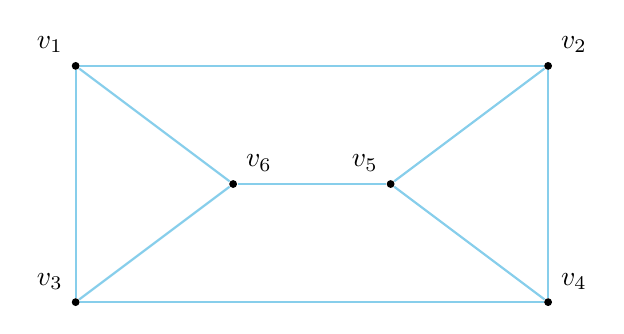
\begin{tikzpicture}[
  start chain=going right,
  roundnode/.style={draw,shape=circle,fill=blue,minimum size=1mm},
  ]
  \tikzset{%
    in place/.style={
      auto=false,
      fill=white,
      inner sep=2pt,
    },
  }
  %Nodes
  \node[circle,fill,inner sep=1pt,label={north west:$v_1$}](v1){};
  \node[circle,fill,inner sep=1pt,label={north east:$v_2$},xshift=5cm](v2)[right of=v1]{};
  \node[circle,fill,inner sep=1pt,label={north west:$v_3$},yshift=-2cm](v3)[below of=v1]{};
  \node[circle,fill,inner sep=1pt,label={north east:$v_4$},yshift=-2cm](v4)[below of=v2]{};
  \node[circle,fill,inner sep=1pt,label={north west:$v_5$},yshift=-0.5cm, xshift=-2cm](v5)[below of=v2]{};
  \node[circle,fill,inner sep=1pt,label={north east:$v_6$},yshift=-0.5cm, xshift=-4cm](v6)[below of=v2]{};
  %Lines
  \draw[-, auto]
    % Straight Line
    (v1) edge[color=SkyBlue, thick](v2)
    (v1) edge[color=SkyBlue, thick](v3)
    (v1) edge[color=SkyBlue, thick](v6)
    (v2) edge[color=SkyBlue, thick](v5)
    (v2) edge[color=SkyBlue, thick](v4)
    (v3) edge[color=SkyBlue, thick](v6)
    (v3) edge[color=SkyBlue, thick](v4)
    (v4) edge[color=SkyBlue, thick](v5)
    (v5) edge[color=SkyBlue, thick](v6)
    ;
\end{tikzpicture}
\subsection*{16 - b}
Yes.
\\ \\
Everyone can be a friend of each other.
Since there are 4 total people, each person could have a maximum of 3 friends. 
In this case where everyone has the maximum, then each person would have exactly 3 friends. 
In other words, every person of a friend of each other.
\\ \\
Let's visualize this.
The vertices $a$, $b$, $c$, and $d$ will represent the 4 people. 
The edges will represent the friendship between each person.
Then in the case where each of the 4 people has exactly 3 friends:
\\ \\
\begin{center}
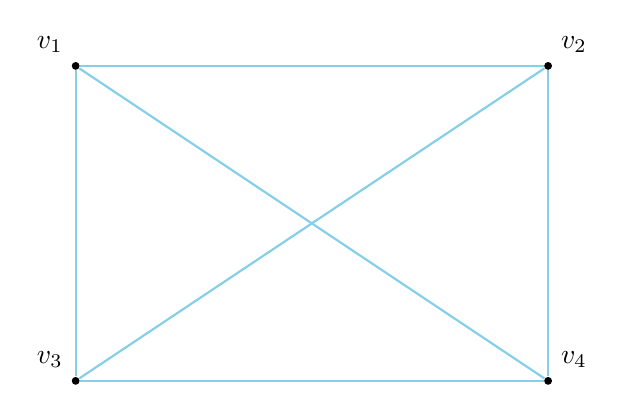
\begin{tikzpicture}[
  start chain=going right,
  roundnode/.style={draw,shape=circle,fill=blue,minimum size=1mm},
  ]
  \tikzset{%
    in place/.style={
      auto=false,
      fill=white,
      inner sep=2pt,
    },
  }
  %Nodes
  \node[circle,fill,inner sep=1pt,label={north west:$v_1$}](v1){};
  \node[circle,fill,inner sep=1pt,label={north east:$v_2$},xshift=5cm](v2)[right of=v1]{};
  \node[circle,fill,inner sep=1pt,label={north west:$v_3$},yshift=-3cm](v3)[below of=v1]{};
  \node[circle,fill,inner sep=1pt,label={north east:$v_4$},yshift=-3cm](v4)[below of=v2]{};
  %Lines
  \draw[-, auto]
    % Straight Line
    (v1) edge[color=SkyBlue, thick](v2)
    (v1) edge[color=SkyBlue, thick](v3)
    (v1) edge[color=SkyBlue, thick](v4)
    (v2) edge[color=SkyBlue, thick](v3)
    (v2) edge[color=SkyBlue, thick](v4)
    (v3) edge[color=SkyBlue, thick](v4)
    ;
\end{tikzpicture}
\end{center}
\subsection*{18}
Yes, see the following graph:
\\ \\
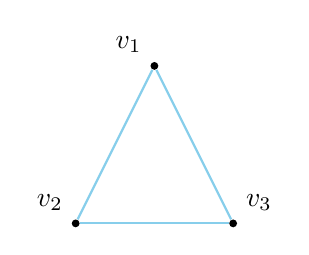
\begin{tikzpicture}[
  start chain=going right,
  roundnode/.style={draw,shape=circle,fill=blue,minimum size=1mm},
  ]
  \tikzset{%
    in place/.style={
      auto=false,
      fill=white,
      inner sep=2pt,
    },
  }
  %Nodes
  \node[circle,fill,inner sep=1pt,label={north west:$v_1$}](v1){};
  \node[circle,fill,inner sep=1pt,label={north west:$v_2$},yshift=-2cm](v2)[left of=v1]{};
  \node[circle,fill,inner sep=1pt,label={north east:$v_3$},yshift=-2cm](v3)[right of=v1]{};
  %Lines
  \draw[-, auto]
    % Straight Line
    (v1) edge[color=SkyBlue, thick](v2)
    (v1) edge[color=SkyBlue, thick](v3)
    (v3) edge[color=SkyBlue, thick](v2)
    ;
\end{tikzpicture}
\newpage
\subsection*{21 - c}
[PROOF BY CONTRADICTION]
\\ \\
\xsupposition
Suppose not. Let $n$ be the number of $v_i$ vertices in the simple graph $K$, and $n \geq 5$.
Then it must be true that all vertices to each have a different degree.
\\ \\
\xgoal
Arrive at contradiction.
\\ \\
\xdeduction
The maximum degree of every vertex $n-1$.
\xlist{
  \item [.] By defintion of simple, each vertex may only to connect to any other vertex once; 
  a vertex may not connect to itself and there may not be multiple connections between any two vertices.
  \item [.] To maximize the degree of each vertex, each vertex must connect to \textit{all other} vertices once.
  \item [.] Therefore, each vertex must have a maximum degree of $n-1$. 
}
\\ \\
Contradiction: It is not possible for all vertices to each have a different degree.
\xlist{
  \item [.] Let's define the vertices such that the first vertex $v_1$ has the highest degree, $v_2$ has the second highest degree, and so on. 
  \item [.] By the previous proof, the higest degree for $v_1$ would be the maximum value $n-1$. Then stepping down by 1 for each vertex; $v_2$ would have a degree of $n-2$, $v_3$ would have a degree of $n-3$, and so on.
  Hence, $v_n$ would then have a degree of $n - (n) = 0$.
  \item [.] However, $deg(v_n) \neq 0$ because the graph is simple.
  \item [.] Therefore we have arrived at contradiction.
}
\\ \\
Therefore, it is contradictory to state that all vertices each have a different degree.
\\ \\
\xconclusion
For any integer $n \geq 5$, it is impossible for all vertices to each have a different degree.
\subsection*{23 - e}
Presume the following defintion from the textbook for a \textbf{complete bipartite graph}:
\\ \\
-------------------------------------------------------------------------------------------------------------------- \\
Let $m$ and $n$ be positive integers. A \textbf{complete bipartite graph} on $(m, n)$ vertices, denoted $K_{m,n}$ is a simple graph whose vertices are divided into two distinct subsets, $V$ with $m$ vertices and $W$ with $n$ vertices, in such a way that:
\begin{itemize}
  \item [i.] Every vertex of $K_{m,n}$ belongs to one of $V$ or $W$, but no vertex belongs to both $V$ and $W$.
  \item [ii.] There is exactly one edge from each vertex of $V$ to each vertex of $W$.
  \item [iii.] There is no edge from any one vertex of $V$ to any other vertex of $V$.
  \item [iv.] There is no edge from any one vertex of $W$ to any other vertex of $W$.
\end{itemize}
\newblock
---------------------------------------------------------------------------------------------------------------------
\\
Let's now count the total number of degrees in $K_{m,n}$. 
\xlist{
  \item [.] By (ii) and (iii), each vertex in $V$ has $n$ connections since each vertex in $V$ is connected to every vertex in $W$.
  \item [.] Since there are $m$ vertices in $V$ and $n$ vertices in $W$, the total number of degrees in $V$ is $mn$.
  \item [.] By (ii) and (iv), each vertex in $W$ has $m$ connections since each vertex in $W$ is connected to every vertex in $n$.
  \item [.] Again, since there are $m$ vertices in $V$ and $n$ vertices in $W$, the total number of degrees in $W$ is $mn$.
  \item [.] Hence, the total number of degrees in $K_{m,n}$ is $deg(V) + deg(W) = mn+mn = 2mn$. 
}
\\ \\
Therefore, the total number of degrees in $K_{m,n}$ is $2mn$.
\subsection*{23 - f}
Since the total number of degrees is $2mn$, and every two degrees comprise its own edge, then the total number of edges is $\frac{2mn}{2} = mn$.
\newpage
\subsection*{24 - d}
This graph is not bipartite.
\\ \\
\xsupposition
Suppose not. Suppose the graph from Exercise 4.9.24, denoted as $F$. Then $F$ must be bipartite.
\\ \\
\xgoal
Arrive at contradiction.
\\ \\
\xdeduction
Denote the defintion of a \textbf{bipartite graph} as follows: 
\\
-------------------------------------------------------------------------------------------------------------------- \\
Let $m$ and $n$ be positive integers. A \textbf{bipartite graph} on $(m, n)$ vertices, denoted $K_{m,n}$ is a simple graph whose vertices are divided into two distinct subsets, $V$ with $m$ vertices and $W$ with $n$ vertices, in such a way that:
\begin{itemize}
  \item [i.] Every vertex of $K_{m,n}$ belongs to one of $V$ or $W$, but no vertex belongs to both $V$ and $W$.
  \item [ii.] There is no edge from any one vertex of $V$ to any other vertex of $V$.
  \item [iii.] There is no edge from any one vertex of $W$ to any other vertex of $W$.
\end{itemize}
\newblock
---------------------------------------------------------------------------------------------------------------------
\\ \\
Contradiction: The vertices $v_2$, $v_3$, and $v_4$ cannot be properly partitioned in the bipartite graph $F$.
\xlist{
  \item [.] In the graph; $v_2$, $v_3$, and $v_4$ are each connected to each other. In other words, each of these three vertices would have a degree of 2 if we werer to exclude all other vertices.
  \item [.] By (i), the vertices $v_2$, $v_3$, and $v_4$ must be between $V$ and $W$.
  \item [.] Yet by (ii) and (iii), there cannot be two vertices in either $V$ or $W$ that are connected to each other.
  \item [.] Since there must be any two of $v_2$, $v_3$, and $v_4$ in the same set, then in either $V$ or $W$ there must be two vertices connected to each other.
  \item [.] Hence, there is a contradiction.
}
\\ \\
Therefore, it is contradictory to state that the vertices $v_2$, $v_3$, and $v_4$ can be properly partitioned in the bipartite graph $F$.
\\ \\
\xconclusion
The graph is not bipartite.
\subsection*{24 - e}
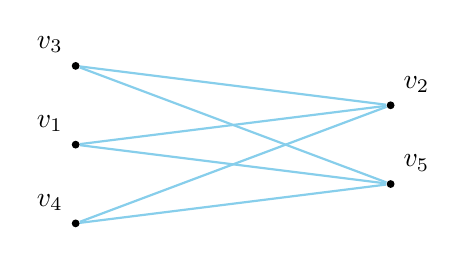
\begin{tikzpicture}[
  start chain=going right,
  roundnode/.style={draw,shape=circle,fill=blue,minimum size=1mm},
  ]
  \tikzset{%
    in place/.style={
      auto=false,
      fill=white,
      inner sep=2pt,
    },
  }
  %Nodes
  \node[circle,fill,inner sep=1pt,label={north west:$v_3$}](v3){};
  \node[circle,fill,inner sep=1pt,label={north west:$v_1$}](v1)[below of=v3]{};
  \node[circle,fill,inner sep=1pt,label={north west:$v_4$}](v4)[below of=v1]{};
  \node[circle,fill,inner sep=1pt,label={north east:$v_2$},xshift=3cm, yshift=-0.5cm](v2)[right of=v3]{};
  \node[circle,fill,inner sep=1pt,label={north east:$v_5$}](v5)[below of=v2]{};
  %Lines
  \draw[-, auto]
    % Straight Line
    (v3) edge[color=SkyBlue, thick](v2)
    (v3) edge[color=SkyBlue, thick](v5)
    (v1) edge[color=SkyBlue, thick](v2)
    (v1) edge[color=SkyBlue, thick](v5)
    (v5) edge[color=SkyBlue, thick](v4)
    (v4) edge[color=SkyBlue, thick](v2)
    ;
\end{tikzpicture}
\\ \\
The nodes on the left column ($v3$, $v1$, and $v4$) are part of $V$ \\ and the nodes on the right column ($v2$ and $v5$) are part of $W$.
\end{document}
